%%% 関西大学 総合情報学部 松下ゼミ 進捗報告 TeXテンプレート Ver 1.1 (2011/12/04) %%%
\documentclass{matsushita-zemi}
\usepackage[dvipdfmx]{graphicx}
\usepackage{comment}
\graphicspath{{./fig/}}

%%% タイトル (長くなる場合は¥¥で適宜改行すること)%%%
\title{HogeHogeにおけるHogeに関する研究}

%%% 氏名 (姓・名の間は半角スペース) %%%
\author{内藤 峻}

\begin{document}
\maketitle

%%% 以下、本文 %%%
\section*{概要}
\label{abstract}
ネットワーク上には多様な種類の情報が存在しており、それらをユーザの要求に応じて適応的にまとめ上げる技術が渇望されている。その一つとして、テキストなどの言語情報と統計データ等の数値情報の相補的な利用に関する研究を行っている。その一環として、本研究では言語情報と数値情報が密接な関係にある株価などの動向情報に着目しそれらを統一的な枠組みで可視化する手法を提案する。株価などの統計情報の場合、その正確な値を知るには数値情報が適切であるのに対して、変動の大局的な理解や背景となる事象の把握には言語情報が適している。そこで、これらを一つのグラフ上に提示し、その情報源に対話的にアクセスできるようにした。

\section{はじめに}
\label{background} 
近年、様々な情報が電子化されネットワーク上に蓄積されている。それに伴い、これらの情報を利用して、意思決定や問題解決に役立てる試みがなされている。しかし、蓄積された情報は情報洪水と言われるほど増加しているうえ、時間の経過に伴って更に増加し続けている。そのため、"情報の在処を見つける"ことを主眼とした検索技術ではユーザの要求に十分に答えることができず、ユーザの意図や関心に応じて適応的に纏め上げ、それへの簡便なアクセスを支援する技術、言うなれば"情報の理解を助ける"技術が渇望されている\cite{Elucignage}。このような背景の下、我々は新聞記事テキストや統計データといった異なるモードの情報を相補的に用いて編纂し、ユーザの情報アクセス行為を容易にする技術の実現を目指している。

ネットワーク上にはテキストだけでなく音声や画像、動画など様々な種類の情報が存在している。将来的にはそれらの情報全てを対象とし、状況や目的に応じて取捨選択やモード変換を行い、適切な形態で組み合わせてユーザに提供することが望まれるが、現状の技術レベルではその実現はよういではない。そこで本研究では、まず時間的変動を伴う統計データ(時系列数位置情報)とそれに関連する記事(言語情報)を対象とし、ユーザがそれらの情報にアクセスしたり、その概要を把握したりする際の支援となる可視化手法について議論する\cite{Elucignage-jsai}。

\section{デザイン指針}
%シナリオに基づいた提案の話

\section{Elucignage プロトタイプシステム}
\subsection{概要}

\subsection{実装}
\begin{comment}
現在、図\ref{LTCond} ならびに図\ref{LCDCond} に示すような二つの実験環
境を作成し、表\ref{exp} に示す 4 群を対象に、被験者間実験をデザインし
ている。実験課題には、迷路上で 1 名の逃亡者を 3 名の追跡者が追いかけて
捕まえるタイプの課題(迷路課題)を用いる。現在、本課題のプログラムを 
Processing で作成しており、クライアント部が完成、サーバ部も 8 割の実装
が完了している。8 月末までにサーバ部を実装し、テストトライアルを行うと
ともに、その結果を反映させた改良を行う。その後、ゼミ外から被験者 80 名
を募集し、本実験を行う。本実験は9月から10月を予定している。
\end{comment}

\section{先行研究}
\label{relatedworks} 

\section{おわりに}

%% 図の挿入 (captionが下)
\begin{figure}[b]
 \centering
 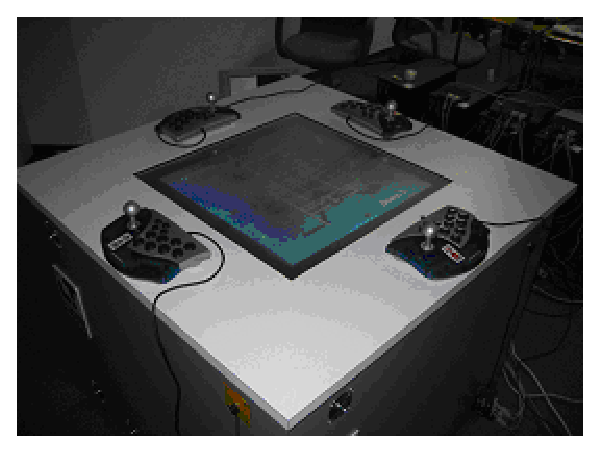
\includegraphics[width=0.4\columnwidth]{LTCond.eps}
 \caption{Lumisight Table 条件}
 \label{LTCond}
\end{figure}

\section{先行研究}
\label{relatedworks} 

%% 表作成 (captionが上)
\begin{table}[p]
\caption{実験群}
\label{exp}
\begin{center}
\begin{tabular}{lcc}
\hline\hline
         & 統制群 1 & 統制群 2\\
\hline
LT 条件  & 20       &   20    \\
LCD 条件 & 20       &   20    \\ 
\hline
\end{tabular}
\end{center}
\end{table}

%%% 参考文献 %%%
\bibliographystyle{ipsjsort}
\bibliography{reference}

\end{document}